\documentclass[psamsfonts,reqno]{amsart}

%-------Packages---------
\usepackage{amssymb,amsfonts}
\usepackage[all,arc]{xy}
\usepackage{enumerate}
\usepackage{mathrsfs}
\usepackage{graphicx}			% Insert images
\usepackage{algorithm}			% Algorithms/pseudocode
\usepackage{algpseudocode}		% Pseudocode
\usepackage{minted}				% Code highlighting
\usepackage{biblatex}			% To create bibliography
\addbibresource{citation.bib}	% Citation reference for bibliography
\usepackage[group-separator={\,}]{siunitx} 	% Formatting numbers (use spaces, not commas)
\newcommand{\Mod}[1]{\ (\mathrm{mod}\ #1)}

%--------Theorem Environments--------
%theoremstyle{plain} --- default
\newtheorem{thm}{Theorem}[section]
\newtheorem{cor}[thm]{Corollary}
\newtheorem{prop}[thm]{Proposition}
\newtheorem{lem}[thm]{Lemma}
\newtheorem{conj}[thm]{Conjecture}
\newtheorem{quest}[thm]{Question}

\theoremstyle{definition}
\newtheorem{defn}[thm]{Definition}
\newtheorem{defns}[thm]{Definitions}
\newtheorem{con}[thm]{Construction}
\newtheorem{exmp}[thm]{Example}
\newtheorem{exmps}[thm]{Examples}
\newtheorem{notn}[thm]{Notation}
\newtheorem{notns}[thm]{Notations}
\newtheorem{addm}[thm]{Addendum}
\newtheorem{exer}[thm]{Exercise}

\theoremstyle{remark}
\newtheorem{rem}[thm]{Remark}
\newtheorem{rems}[thm]{Remarks}
\newtheorem{warn}[thm]{Warning}
\newtheorem{sch}[thm]{Scholium}

\makeatletter
\let\c@equation\c@thm
\makeatother
\numberwithin{equation}{section}

\bibstyle{plain}

%--------Meta Data: Fill in your info------
\begin{document}

\title{Large Integer Multiplication:\\A Friendly Survey of Algorithms}
\date{December 8, 2023}

\author{JT Miller}
\address{University of Illinois at Springfield}
\thanks{jt.miller@txbinary.com}
\email{jt.miller@txbinary.com}

\begin{abstract}

How do computers multiply integers larger than the number of bits within dedicated hardware? This paper provides a survey of several large integer multiplication algorithms that answer this question. The aim of the paper is to provide a friendly introduction with many examples such that undergraduate students can look past the complexity of these algorithms, grasp the fundamentals, and hopefully understand some of the beauty and wonder in the algorithms. 

\end{abstract}

\maketitle


\tableofcontents

\section{Introduction}

Large integer multiplication is pervasive in our lives in the form of cryptography. One need only look at the innards of any crypto library to find a BigInt library or API behind the scenes. Within those libraries/APIs are the algorithms discussed within this paper. There are other less pervasive uses, such as scientific and algorithm research, large-scale data analysis, and of course computational mathematics. 

How do computers multiply integers larger than the number of bits within dedicated hardware? This paper provides a survey of several large integer multiplication algorithms that answer this question. The aim of the paper is to provide a friendly introduction with many examples such that undergraduate students can look past the complexity of these algorithms, grasp the fundamentals, and hopefully understand some of the beauty in the algorithms. 

The title of the paper is a tribute to Dr. Silverman's wonderful \textit{A Friendly Introduction to Number Theory}. We will start with grade school multiplication, then cover a simple but useful extension that allows multiplication in ``chunks''. We then cover the first advance in nearly 4000 years \cite{burton1985history}, Karatsuba's algorithm. Next we will discuss the Toom-Cook algorithm that is a generalization of Karatsuba's algorithm. Next we cover the fundamentals of the Discrete Fourier Transform (DFT) and Fast Fourier Transform (FFT) to understand how these algorithms are used to multiply large integers. Finally, we cover the Sch\"{o}nhage-Strassen multiplication algorithm, which gets us to $\mathcal{O}(n \log n \log \log n)$ time complexity.

\subsection{Prerequisites}
There are surprisingly few prerequisites to understand this material. Perhaps the most important prerequisite is some familiarity with mathematical notation. Otherwise, grade school arithmetic and trigonometry through complex numbers and the unit circle is all that is required. The more advanced algorithms would benefit from familiarity with matrix manipulation, Linear Algebra, and Calculus, but these are not strict prerequisites. As this is a friendly introduction, we have tried to make the algorithms available to the widest audience possible, and hence avoided discussions that require more advanced mathematics. Suggestions to make the material available to an even wider audience are welcome.

\subsection{Software}
The companion software for this paper can be found on GitHub at (TODO: Insert github link here) and GitLab at (TODO: Insert gitlab link here). All of the examples shown are solved in software and stepped through, as well as all algorithms illustrated. Most programs were initially done in Python as support for large integer arithmetic is built into the language which makes testing easy, but the programs are also available (to some extent) in Java, MATLAB, and C/C++. 

\section{Grade School Multiplication}
Multiplication dates back to at least 2000 B.C. \cite{burton1985history} and of course we all learn how to multiply integers in grade school. A review of this algorithm gives us a grasp of the terminology and notation we will use throughout the rest of this paper to discuss multiplication algorithms. We start with a representation for integers, which will be useful for later algorithms.

\subsection{Integer Representation \nopunct}

We can express any positive integer $x$ as a summation of coefficients raised to a base power \cite{silverman2014friendly}:
\begin{equation}
	x = \sum_{i=0}^{n-1} X_iB^i.
\end{equation}
Given a base system and coefficients, we can express $x$ as a coefficient vector with $n$ entries: 
\begin{equation}
	\mathbf{X}=\{X_0, X_1, X_2, ..., X_{n-1}\}.
\end{equation}
E.g. we can represent the number $40342$ as 
\begin{equation}
	\mathbf{X}=\{2, 4, 3, 0, 4\}
\end{equation}
and in base 10 we would have 
\begin{equation}
	2 \cdot 10^0 + 4 \cdot 10^1 + 3 \cdot 10^2 + 0 \cdot 10^3 + 4 \cdot 10^4 =40342.
\end{equation}

Note that our coefficients for powers appear ``backward'' in the set/array, as lower-powered coefficients appear first, but we naturally write higher-power to lower-power coefficients left to right when expressing numbers. Even from this simple idea, we can make a few observations that will prove useful later. Given two positive integers $x$ and $y$, with one integer having fewer coefficients, we can still express the integers as vectors of the same length by zero-padding the smaller integer. E.g. let $x=389$ and $y=4$, then we can simply say $\mathbf{X}=\{9, 8, 3\}$ and $\mathbf{Y}=\{4, 0, 0\}$. If the larger integer has $n$ coefficients, we now have two integers with $n$ coefficients.

How many coefficients are necessary to store the result of two $n$-digit positive integers? 
\begin{lem}
	Multiplying two $n$-digit positive integers requires no more than $2n$ coefficients. 
\end{lem}
\begin{proof}
	Let $x$ be an $n$-digit positive integer in positive base $B$. 
	\begin{align}
		x & \leq B^n-1 \\
		x^2 & \leq ({B^n-1})^2 \\
		x^2 & \leq B^{2n} - 2B^n + 1 \label{max_base_number}
	\end{align}
	$2B^n > 1$ for all $B>0$, so we may simplify the right side of equation~\ref{max_base_number} to 
	\begin{align}
		x^2 & < B^{2n}
	\end{align}
\end{proof}
Let's work an example multiplying $9999 \times 9999 = 99980001$ in base 10. We have $B=10$ and $n=4$. In this case, we are using the maximum value ($9999$) that can be represented in base 10 with 4 digits. We can simply use equation~\ref{max_base_number} directly and compute $x^2$.
\begin{align*}
	x^2 &= B^{2n} - 2B^n + 1 \\
	x^2 &= 10^8 - 2 \cdot 10^4 + 1 \\
	x^2 &= 99980001
\end{align*}

Let us now discuss our (modified) grade school multiplication algorithm.

\subsection{Algorithm \nopunct}

For grade school multiplication, let us use the values $x=123$ and $y=789$ to illustrate our algorithm. Instead of simply multiplying the ones' digits $9$ and $3$ and writing the new ones' digit $7$ and carrying the $2$, we will write the individual products in each ``column'' corresponding to the base power, as shown in Figure~\ref{fig:gs01}. After we have computed all partial products, we add the partial products within each ``column'' or base power. Finally, we carry any overflow of partial products to the next column/base power, and we have our summation of final products yielding the answer $97047$. 
\begin{figure}[H]
	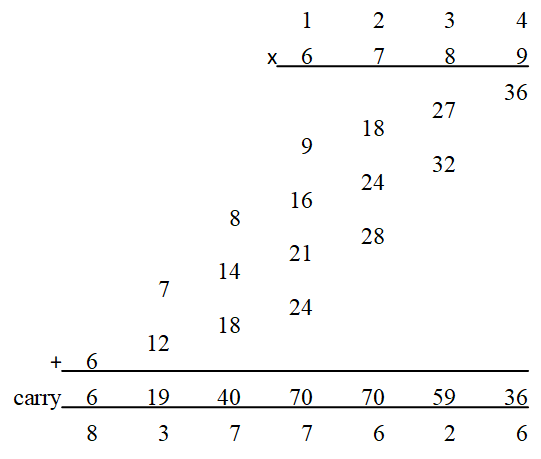
\includegraphics{img/gs_multiplication_ex_01}
	\caption{Grade School Multiplication of $123 \times 789$}
	\label{fig:gs01}
\end{figure}

Expressed mathematically, we are performing the following,
\begin{equation}
	\label{gsmul}
	xy = \sum_{k=0}^{n-1}\sum_{j=0}^{n-1}X_jY_kB^{j+k}.
\end{equation}

Now, let us determine an algorithm for performing our grade school multiplication. 
\begin{algorithm}[H]
	\caption{Grade School Multiplication}
	\label{gs_mult_algo}
	\begin{algorithmic}
	\For{$j \in \{0,1,...,n-1\}$}
		\For{$k \in \{0,1,...,n-1\}$}
			\State {$W[j+k] += X_jY_kB^{j+k}$}
		\EndFor
	\EndFor
	\State $c = 0$
	\For{$j \in \{0,1,...,2n-2\}$}
		\State $c = W[j] \Mod{B}$				
		\State $W[j] = \lfloor W[j] / B \rfloor$
		\State $W[j+1] += c$
	\EndFor
	\State return $W$
\end{algorithmic}
\end{algorithm}

\subsection{Time Complexity Analysis \nopunct}

We will not belabor the time-complexity analysis to determine exact counts of the operations involved. In general additions are easier for computers, so we will typically only care about the number of necessary multiplications. From Figure~\ref{fig:gs01} we can see that for $n$ digits, we have $n \times n$ partial products to compute. Accordingly, our grade school multiplication algorithm yields $\mathcal{O}(n^2)$.

\subsection{Code Examples \nopunct}

\begin{minted}[fontsize=\footnotesize]{python}
def left_to_right(x: list[int]) -> str:
    """Take a least significant first digit set and return a string representation
    of the number."""
    return "".join(str(d) for d in x[::-1])
    
def zero_pad(x: list[int], n: int, pad: int=0) -> list[int]:
    """Zero pad a list to the given length."""
    return [pad] * (n - len(x)) + x

def grade_school_multiplication(X: list[int], Y: list[int]) -> list[int]:
    # Pad the shorter list with zeros to match the lengths
    n = max(len(X), len(Y))
    X = zero_pad(X, n)
    Y = zero_pad(Y, n)

    # Initialize the result list W with zeros, length should be 2 * n
    W = [0] * (2 * n)

    # Multiply all partial products and add them to W
    for j in range(len(X)):
        for k in range(len(Y)):
            W[j + k] += X[j] * Y[k]

    # Handle carries from least significant to most significant digit
    for i in range(len(W) - 1):
        carry, W[i] = divmod(W[i], 10)
        W[i + 1] += carry

    # Remove excess leading zeros, if any, but leave at least one digit
    while len(W) > 1 and W[-1] == 0:
        W.pop()

    return W
\end{minted}

\section{Chunky Grade School Multiplication}

We can make a simple modification to our grade school multiplication that allows us to increase our multiplication speed by a factor of our machine's bit-length. Because this technique is generic, the exact bit-lengths involved in integer hardware multiplication aren't necessarily important. The increase comes by recognizing that instead of multiplying a single digit at a time, we can multiply chunks of digits. We will use $\num{123456} \times \num{987654} = \num{121931812224}$ to illustrate\footnote{Note that the spaces in numbers such as these are strictly for readability purposes. Numbers formatted with spaces like those in the previous multiplication are still single contiguous numbers.} our chunky grade school multiplication algorithm improvement.

Figure~\ref{fig:cgs01} shows how we can group our digits into chunks. These chunks allow fewer partial products even though we now have more total digits. The chunks ``skip'' base powers by grouping digits. 
 \begin{figure}[H]
	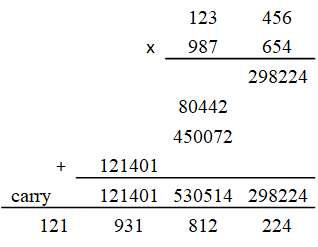
\includegraphics{img/chunky_gs_mul_ex_01}
	\caption{Chunky Grade School Multiplication of $\num{123456} \times \num{987654}$}
	\label{fig:cgs01}
\end{figure}

If we group 3 digits then we are using a chunk size of 3 base powers, which we then keep track of throughout the algorithm. In actual large integer multiplication algorithms, we must be careful to guarantee that the summation of partial products for a given base power/column fits within the machine word size/bit width. Let us use the positive integer $h$ for chunk size, then we have just a small modification from equation~\ref{gsmul}, 
\begin{equation}
	xy = \sum_{k=0}^{n-1}\sum_{j=0}^{n-1}X_jY_kB^{h(j+k)}.
\end{equation}

\subsection{Algorithm \nopunct}

\begin{algorithm}[H]
	\caption{Chunkify}
	\label{chunkify}
	\begin{algorithmic}
		\State Pick a chunk size $h > 1$
		\State Pad $X, \; Y$ to $kh$ where $k$ is a positive integer
		\State $n = len(X)/h$
		\State $X_{chunky} = \{0, 0, ..., 0\}$
		\State $Y_{chunky} = \{0, 0, ..., 0\}$
		\For{$j \in \{0,1,...,nh-1\}$}
			\State $X_{chunky}[\lfloor j/h \rfloor] += X[j] * 10^{j \Mod{h}}$
			\State $Y_{chunky}[\lfloor j/h \rfloor] += X[j] * 10^{j \Mod{h}}$
		\EndFor
		\State return $X_{chunky}, \; Y_{chunky}$
	\end{algorithmic}
\end{algorithm}

\begin{algorithm}
	\caption{Chunky Grade School Multiplication}
	\label{chunky_gs_mult_algo}
	\begin{algorithmic}
		\For{$j \in \{0,1,...,n-1\}$}
			\For{$k \in \{0,1,...,n-1\}$}
				\State {$W[j+k] += X_jY_kB^{j+k}$}
			\EndFor
		\EndFor
		\State $c = 0$
		\For{$j \in \{0,1,...,2n-2\}$}
			\State $c = W[j] \Mod{B^h}$				
			\State $W[j] = \lfloor W[j] / B^h \rfloor$
			\State $W[j+1] += c$
		\EndFor
		\State return $W$
	\end{algorithmic}
\end{algorithm}

\subsection{Time Complexity Analysis \nopunct}

From Figure~\ref{fig:cgs01} we can see that we have reduced from $n \times n$ operations to $n/h \times n/h$ operations, which can be a significant real reduction, but still results in a run time of $\mathcal{O}(n^2)$.

\subsection{Code Examples \nopunct}

\begin{minted}[fontsize=\footnotesize]{python}
def chunkify(x: list[int], h: int) -> list[int]:
    """Split a list into chunks of size n."""
    if len(x) % h != 0:
        raise ValueError(f"Length of list must be a multiple of {h}, \
        	{len(x)} is not!")
    n = len(x) // h
    chunks = [0] * n
    for ix, val in enumerate(x):
        chunks[ix // h] += val * 10 ** (ix % h)
    return chunks


def chunky_grade_school_multiplication(
	X: list[int], Y: list[int], h: int
) -> list[int]:
    # Pad the shorter list with zeros to match the lengths
    n = max(len(X), len(Y))
    X = zero_pad(X, n)
    Y = zero_pad(Y, n)

    # Verify X and Y are chunkable
    if len(X) % h != 0:
        raise ValueError(f"Length of X must be a multiple of {h}, \
        	{len(X)} is not!")

    # Chunkify X and Y
    X = chunkify(X[:], h)
    Y = chunkify(Y[:], h)

    n = len(X_chunks)

    # Initialize the result list W with zeros, length should be 2 * n
    W = [0] * (2 * n)

    # Multiply all partial products and add them to W
    for j in range(len(X)):
        for k in range(len(Y)):
            W[j + k] += X[j] * Y[k]

    # Handle carries from least significant to most significant digit
    for i in range(len(W) - 1):
        carry, W[i] = divmod(W[i], 10**h)
        W[i + 1] += carry

    # Remove excess leading zeros, if any, but leave at least one digit
    while len(W) > 1 and W[-1] == 0:
        W.pop()

    return W
\end{minted}

\section{Karatsuba}
We now turn our attention to Karatsuba's algorithm. In 1960, Andrey Kolmogorov conjectured that $\mathcal{O}(n^2)$ was as fast as multiplication could be achieved. Kolmogorov held a seminar at Moscow University where he presented this and other conjectures. Anatoly Karatsuba, a 23-year-old student, found a divide and conquer deconstruction method that multiplies integers in $\mathcal{O}(n^{\log_2 3})$ that he presented at the next seminar, which Kolmogorov then disbanded (TODO: INSERT REFERENCE HERE). Kolmogorov was so impressed with Karatsuba's algorithm that he wrote a paper for him, which Karatsuba only became aware of after the edits were mailed back to him \cite{karatsuba1995complexity}. Perhaps the best way to motivate some is to say that something is impossible.

\subsection{Algorithm \nopunct}
Karatsuba's algorithm involves manipulating the partial products involved in multiplication, a divide and conquer approach. Let the tens' and ones' digits of $x$ to be $ab$, or $X_1 = a$, and $X_0 = b$ from our previous discussions. Similarly, let the tens and ones' digits of $y$ be $cd$, or $Y_1 = c$ and $Y_0 = d$. Figure~\ref{fig:gs_abcd} shows this simple grade school multiplication. 
\begin{figure}[H]
	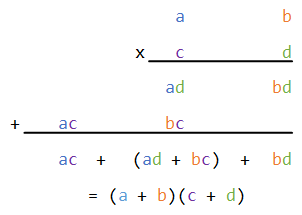
\includegraphics{img/gs_abcd}
	\caption{Grade School $abcd$ Multiplication}
	\label{fig:gs_abcd}
\end{figure}

Note that we are neglecting the base. Figure~\ref{fig:gs_abcdz} shows the same multiplication with our base $z$ included. 
\begin{figure}[H]
	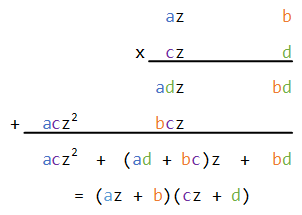
\includegraphics{img/gs_abcdz}
	\caption{Grade School $abcdz$ Multiplication (includes base $z$)}
	\label{fig:gs_abcdz}
\end{figure}

Karatsuba recognized that the multiplication of partial products, $(a+b)(c+d)=ac+(ad+bc)+bd$ could be manipulated to yield three multiplications instead of four. $ac$ is one multiplication, $bd$ is the second, and then we can use the fact that $(ad+bc) = (a+b)(c+d) - (ac + bd)$ for the third multiplication. We now have all the partial products necessary, having deconstructed the addition of partial products. At the cost of a few more additions and subtractions, we can remove one multiplication. Figure~\ref{fig:abcd_equation} shows this simple coefficient manipulation with the multiplications numbered at the bottom of equations and the ``free'' multiplication shown. The letters $A$-$E$ denote the arithmetic quantities we will compute during the algorithm.
\begin{figure}[H]
	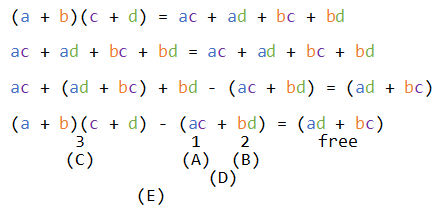
\includegraphics{img/abcd_equation}
	\caption{Karatsuba's Manipulation of Coefficients}
	\label{fig:abcd_equation}
\end{figure}

Figure~\ref{fig:karatsuba_example} shows an example for $\num{25786109} \times \num{72166948} = \num{1860904787325332}$ with the same coloring used to denote $abcd$ as the previous explanations. Note that we have combined the algorithm with chunking (typically this is referred to as blocking, but the term chunking is more fun) that combines several coefficients. 
\begin{figure}[H]
	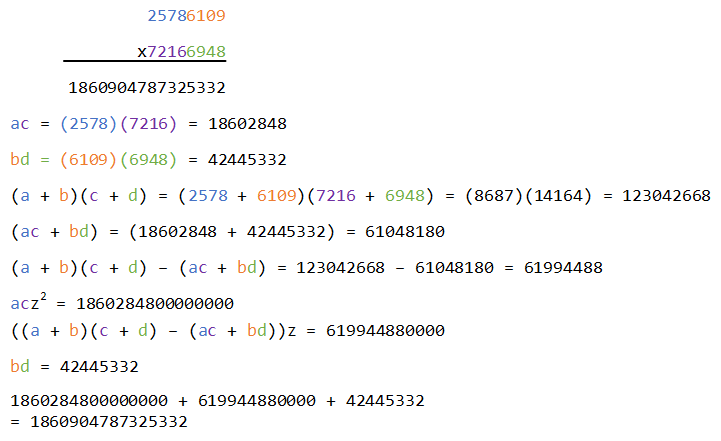
\includegraphics{img/karatsuba_example}
	\caption{Karatsuba Example}
	\label{fig:karatsuba_example}
\end{figure}

Karatsuba's three coefficient products, $ac$, $bd$, and $(a+b)(c+d)$, can be used to recursively subdivide the problem further. Figure~\ref{fig:karatsuba_large_example} shows a larger Karatsuba example where we recursively apply Karatsuba to coefficients.\footnote{The recursion is for illustrative/instructive purposes and unnecessary. We could have used more coefficients and a larger base power without the recursive stages.} The equations in the upper right are those as before. The numbers $1$-$3$ show the three multiplications and the letters  $A$-$E$ to denote the arithmetic quantities computed during the algorithm. We shows these $A$-$E$ quantities under each stage, including the final summation with base powers multiplied into computed quantities. Note that we dispense with printing this final summation after the first stage as the large quantities become cumbersome to print and we just print the $A$-$E$ quantities and final result. \cite{wiki:Karatsuba_algorithm} provides an excellent graphic with another example and a different representation of the computations involved.
\begin{figure}[H]
	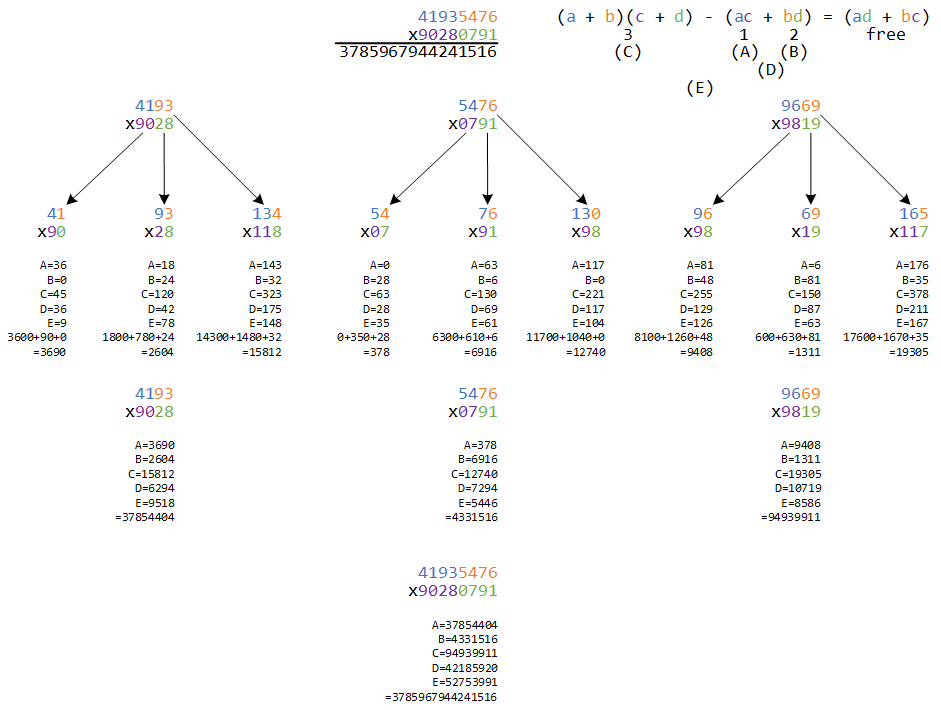
\includegraphics{img/karatsuba_large_example}
	\caption{Larger Karatsuba Example}
	\label{fig:karatsuba_large_example}
\end{figure}

(TODO: Add algorithm)

\subsection{Time Complexity Analysis \nopunct}

As we noted above, because Karatsuba allows recursively subdividing the problem in half, using three coefficient multiplications, the runtime is $\mathcal{O}(n^{\log_2{3}})$. $\log_2{3} \approxeq 1.585$, so the runtime complexity of Karatsuba's algorithm is commonly referred to as $\mathcal{O}(n^{1.585})$. 

\subsection{Code Examples \nopunct}

(TODO: Add python for real algorithm and discussion)

\begin{minted}[fontsize=\footnotesize]{matlab}
function [] = karatsuba(x, y, n)
	a = floor(x/10^n);
	b = mod(x,10^n);
	c = floor(y/10^n);
	d = mod(y,10^n);
	
	A = a*c;
	B = b*d;
	C = (a+b)*(c+d);
	D = A+B;
	E = C - D;
	result = A*10^(2*n) + E*10^n + B;
	fprintf("A=%d\n", A);
	fprintf("B=%d\n", B);
	fprintf("C=%d\n", C);
	fprintf("D=%d\n", D);
	fprintf("E=%d\n", E);
	fprintf("%d+%d+%d\n", A*10^(2*n), E*10^n, B);
	fprintf("=%d\n\n", result);
end	
\end{minted}

\section{Toom-Cook}

The Toom-Cook algorithm generalizes the divide and conquer approach used in Karatsuba. Instead of splitting the multiplicands into two parts, Toom-Cook splits the multiplication into $r$ parts. Toom-Cook then uses the splits as coefficients in a polynomial, as we have done before. The clever part of Toom-Cook is to use these splits parts in the $X$ and $Y$ coefficients to represent polynomials $x(t)$ and $y(t)$, then multiply those polynomials together. Because the $x(t)$ and $y(t)$ polynomials will be of degree $r-1$, their product will be of degree $r-2$, at most. We can evaluate the multiplication of $x(t)$ and $y(t)$ at $2r-1$ points to recover the product $w(t)$, of degree $2r-2$. Hence we are now multiplying together polynomials to recover integers! 

Judicious selection of $r$ and the points at which we multiply the polynomials yields the best results. Toom-Cook multiplication of $n$-word numbers takes, at best, $\mathcal{O}(n^{1+1/\sqrt{\log{n}}})$ \cite{brent2010modern}.

Consider that we pad the multiplicands so that we can split the multiplicand into three coefficients of equal length. We can then write our multiplicands as polynomials
\begin{align*}
	x(t) &= x_2t^2 + x_1t + x_0 \\
	y(t) &= y_2t^2 + y_1t + y_0.
\end{align*}

We multiply these two polynomials to produce $w(t)$:
\begin{equation*}
	w(t)=x(t)*y(t).
\end{equation*}

Because we know the maximum degree of $w(t)$, we can write the polynomial's representation as
\begin{equation*}
	w(t) = w_4t^4 + w_3t^3 + w_2t^2 + w_1t + w_0.
\end{equation*}

We should note that $t$ is equivalent to our base, which of course may be ``chunks''. Hence $t = B^h$, and $t^k = B^{kh}$ where $k$ is some positive integer. Obviously, $w_4 = x_2y_2$, and so on:
\begin{align*}
	w_4 &= x_2y_2 \\
	w_3 &= x_2y_1 + x_1y_2 \\
	w_2 &= x_2y_0 + x_1y_1 + x_0y_2 \\
	w_1 &= x_1y_0 + x_0y_1 \\
	w_0 &= x_0y_0.
\end{align*}

For the Toom-Cook algorithm split into 3 parts, a popular choice for the points is $0$, $1$, $-1$, $-2$, and $\infty$. The point at infinity simply reduces to the highest level coefficient. Our equations reduce nicely using these points:
\begin{align*}
	x(0) &= x_2(0)^2 + x_1(0) + x_0 &&= x_0 \\
	x(1) &= x_2(1)^2 + x_1(1) + x_0	&&= x_2 + x_1 + x_0 \\
	x(-1) &= x_2(-1)^2 + x_1(-1) + x_0 &&= x_2 - x_1 + x_0 \\
	x(-2) &= x_2(-2)^2 + x_1(-2) + x_0 &&= 4x_2 - 2x_1 + x_0 \\
	x(\infty) &= x_2(\infty)^2 + x_1(\infty) + x_0 &&= x_2.
\end{align*}

We can further optimize the above arithmetic computations by saving some partially computed results\footnote{Note that $\gamma$ is simply a variable we use for the partial computation of $x_0 + x_2$, there is no other significance.} and applying to subsequent arithmetic computations:
\begin{align}
	\gamma &= x_0 + x_2 \label{toom_opt1} \\
	x(0) &= x_0 \label{toom_opt2} \\
	x(1) &= \gamma + x_1 \label{toom_opt3} \\
	x(-1) &= \gamma - x_1 \label{toom_opt4} \\
	x(-2) &= 2(x(-1) + x_2) - x_0 \label{toom_opt5} \\
	x(\infty) &= x_2. \label{toom_opt6}
\end{align}

The same computations are used for $y(t)$. Now we can compute $w(t) = x(t)y(t)$. At this point, we will introduce some linear algebra that compactly shows the $2r-1$ equations we are solving and how we can obtain $w(t)$ (and the $W$s we are after) by inverting this matrix. For those unfamiliar with linear algebra, you can skip down below to where we restate $w(t)$. You can solve the simultaneous set of equations to arrive at the same point.
\begin{align*}
	\begin{pmatrix}
		w(0) \\ 
		w(1) \\
		w(-1) \\
		w(-2) \\
		w(\infty)
	\end{pmatrix}
	&=
	\begin{pmatrix}
		0^0 & 0^1 & 0^2 & 0^3 & 0^4 \\
		1^0 & 1^1 & 1^2 & 1^3 & 1^4 \\
		(-1)^0 & (-1)^1 & (-1)^2 & (-1)^3 & (-1)^4 \\
		(-2)^0 & (-2)^1 & (-2)^2 & (-2)^3 & (-2)^4 \\
		0 & 0 & 0 & 0 & 1
	\end{pmatrix}
	\begin{pmatrix}
		w_0 \\
		w_1 \\
		w_2 \\
		w_3 \\
		w_4
	\end{pmatrix}
	\\
	&=
	\begin{pmatrix}
		1 & 0 & 0 & 0 & 0 \\
		1 & 1 & 1 & 1 & 1 \\
		1 & -1 & 1 & -1 & 1 \\
		1 & -2 & 4 & -8 & 16 \\
		0 & 0 & 0 & 0 & 1
	\end{pmatrix}
	\begin{pmatrix}
		w_0 \\
		w_1 \\
		w_2 \\
		w_3 \\
		w_4		
	\end{pmatrix}
	.
\end{align*}

Because we were judicious in the choice of our evaluation points, the matrix above is invertible, and we may simply invert the matrix to solve for our coefficients directly.
\begin{align*}
	\begin{pmatrix}
		w_0 \\
		w_1 \\
		w_2 \\
		w_3 \\
		w_4		
	\end{pmatrix}
	& =
	\begin{pmatrix}
		1 & 0 & 0 & 0 & 0 \\
		1 & 1 & 1 & 1 & 1 \\
		1 & -1 & 1 & -1 & 1 \\
		1 & -2 & 4 & -8 & 16 \\
		0 & 0 & 0 & 0 & 1
	\end{pmatrix}^{-1}
	\begin{pmatrix}
		w(0) \\ 
		w(1) \\
		w(-1) \\
		w(-2) \\
		w(\infty)
	\end{pmatrix}
	\\
	&=
	\begin{pmatrix}
		1 & 0 & 0 & 0 & 0 \\
		1/2 & 1/3 & -1 & 1/6 & -2 \\
		-1 & 1/2 & 1/2 & 0 & -1 \\
		-1/2 & 1/6 & 1/2 & -1/6 & 2 \\
		0 & 0 & 0 & 0 & 1
	\end{pmatrix}
	\begin{pmatrix}
		w(0) \\ 
		w(1) \\
		w(-1) \\
		w(-2) \\
		w(\infty)
	\end{pmatrix}	
\end{align*}

For our friends without linear algebra rejoining us, this is
\begin{align*}
	w_0 &= w(0) \\
	w_1 &= \frac{1}{2}w(0) + \frac{1}{3}w(1) - w(-1) + \frac{1}{6}w(-2) -2w(\infty) \\
	w_2 &= -w(0) + \frac{1}{2}w(1) + \frac{1}{2}w(-1) -w(\infty) \\
	w_3 &= -\frac{1}{2}w(0) + \frac{1}{6}w(1) + \frac{1}{2}w(-1) - \frac{1}{6}w(-2) + 2w(\infty) \\
	w_4 &= w(\infty)
\end{align*}

Note that we could optimize this by computing partial summations and then reusing results as we did in Equation~\ref{toom_opt1}-\ref{toom_opt6}. We leave this as an exercise for the reader. Let us compute a Toom-3 example with $\num{698310488572646777019184} \times \num{144585992498882884065634} = 
\num{100965915062655948833325499910140535809533122656}$. Here,
\begin{align*}
	x_2 &= \num{69831048} \\
	x_1 &= \num{85726467} \\
	x_0 &= \num{77019184} \\
	y_2 &= \num{14458599} \\
	y_1 &= \num{24988828} \\
	y_0 &= \num{84065634}.
\end{align*}

Now we can compute our points for our x and y polynomials:
\begin{align*}
	x(0) &= x_0 &&= \num{77019184} \\
	x(1) &= x_2 + x_1 + x_0 &&= \num{69831048} + \num{85726467} + \num{77019184} &&= \num{232576699} \\
	x(-1) &= x_2 - x_1 + x_0 &&= \num{69831048} - \num{85726467} + \num{77019184} &&= \num{61123765} \\
	x(-2) &= 4x_2 - 2x_1 + x_0 &&= 4 \cdot \num{69831048} - 2 \cdot \num{85726467} + \num{77019184} &&= \num{184890442} \\
	x(\infty) &= x_2 &&= \num{85726467} \\ \\
	y(0) &= y_0 &&= \num{84065634} \\
	y(1) &= y_2 + y_1 + y_0 &&= \num{14458599} + \num{24988828} + \num{84065634} &&= \num{123513061} \\
	y(-1) &= y_2 - y_1 + y_0 &&= \num{14458599} - \num{24988828} + \num{84065634} &&= \num{73535405} \\
	y(-2) &= 4y_2 - yx_1 + y_0 &&= 4 \cdot \num{14458599} - 2 \cdot \num{24988828} + \num{84065634} &&= \num{91922374} \\
	y(\infty) &= y_2 &&= \num{14458599}.
\end{align*}

And then multiply the two polynomials points' together to yield points for $w(t)$:
\begin{align*}
	w(0) &= x(0)y(0) &&= \num{77019184} \cdot \num{123513061} &&= \num{6474666533122656}\\
	w(1) &= x(1)y(1) &&= \num{232576699} \cdot \num{73535405} &&= \num{28726260010765639} \\
	w(-1) &= x(-1)y(-1) &&= \num{61123765} \cdot \num{84065634}  &&= \num{4494760814399825} \\
	w(-2) &= x(-2)y(-2) &&= \num{77019184} \cdot \num{91922374} &&= \num{16995568358549308} \\
	w(\infty) &= x(\infty)y(\infty) &&= \num{184890442} \cdot \num{14458599} &&= \num{1009659120781752}.
\end{align*}

We then multiply our inverse matrix by $w(t)$'s points to yield the coefficients:
\begin{align*}
	w_0 &= \num{6474666533122656} \\
	w_1 &= \num{9131268940611430} \\
	w_2 &= \num{9126184758678324} \\
	w_3 &= \num{2984480657571477} \\
	w_4 &= \num{1009659120781752}.
\end{align*}

Now we perform the carries based on our chunk size. We used a chunk of $8$, hence we carry beyond $10^8$ digits of each chunk to the next chunk. As an example, for $w_0$, the lower 8 digits are $\num{33122656}$ and we carry and add $\num{64746665}$ to the lower $8$ digits of the next chunk, $\num{40611430}$, giving us $\num{64746665} + \num{40611430} = \num{105358095}$. Hence the lower $16$ digits of our product are ${0535809533122656}$. We continue in this manner to find our final answer of $\num{698310488572646777019184} \times \num{144585992498882884065634} =\\ 
\num{100965915062655948833325499910140535809533122656}$.

\subsection{Algorithm \nopunct}

TODO: Toom-Cook Algorithm

\subsection{Time Complexity Analysis \nopunct}

TODO: Toom-Cook Analysis

Note how quickly the number of terms grows as we partition our multiplicands into larger numbers. In most cases, this limits the practical use of Toom-Cook to three or four partitions.

\subsection{Code Examples \nopunct}

\begin{minted}[fontsize=\footnotesize]{python}
def pad(x: str, h: int) -> str:
    r = len(x) % h
    if r != 0:
        padding = ['0'] * (h - r)
        return "".join(padding) + x
    return x


def chunkify(x: str, h: int) -> list[int]:
    if len(x) % h != 0:
        print(f"Length of {x} is not an integer multiple of {h}, exiting")
        exit(1)
    return [int(x[max(i - 8, 0):i]) for i in range(len(x), 0, -8)]


def print_coeffs(chunks: list[int], coeff: str = 'x') -> None:
    for ix, chunk in enumerate(chunks):
        print(f"{coeff}_{ix} = {chunk}")


def eval_input_poly(x: list[int]) -> list[int]:
    """x is the coefficients, returns a list of values at our chosen Toom-3 points.
    The points are {0, 1, -1, -2, \infty}"""
    gamma = x[0] + x[2]
    x_of_zero = x[0]
    x_of_one = gamma + x[1]
    x_of_minus_one = gamma - x[1]
    x_of_minus_two = 2*(x_of_minus_one + x[2]) - x[0]
    x_of_infty = x[2]
    x_of_t = [x_of_zero, x_of_one, x_of_minus_one, x_of_minus_two, x_of_infty]
    return x_of_t


def multiply_points(x: list[int], y: list[int]) -> list[int]:
    w = [0] * len(x)
    for ix in range(len(x)):
        w[ix] = x[ix]*y[ix]
    return w


def print_points(x: list[int], var: 'str') -> None:
    print(f"{var}(0)   = {x[0]}")
    print(f"{var}(1)   = {x[1]}")
    print(f"{var}(-1)  = {x[2]}")
    print(f"{var}(-2)  = {x[3]}")
    print(f"{var}(inf) = {x[4]}")


def interp_w(p: list[int]) -> list[int]:
    """p is the list of points for w"""
    w = [0] * 5
    w[0] = p[0]
    w[1] = (1/2)*p[0] + (1/3)*p[1] - p[2] + (1/6)*p[3] - 2*p[4]
    w[2] = -p[0] + (1/2)*p[1] + (1/2)*p[2] - p[4]
    w[3] = -(1/2)*p[0] + (1/6)*p[1] + (1/2)*p[2] - (1/6)*p[3] + 2*p[4]
    w[4] = p[4]
    for ix in range(len(w)):
        w[ix] = int(w[ix])
    return w

def do_carries(w: list[int], h: int) -> list[int]:
    for ix in range(len(w)-1):
        c, w[ix] = divmod(w[ix], 10**h)
        w[ix+1] += c
    return w


def print_num(num: list[int], var: str = 'w') -> None:
    print(f"{var} = {''.join([str(x) for x in num[::-1]])}")


if __name__ == "__main__":
    h = 8

    x = "698310488572646777019184"
    y = "144585992498882884065634"
    x = pad(x, h)
    y = pad(y, h)
    print(f"x = {x}")
    x_chunks = chunkify(x, h)
    print_coeffs(x_chunks, 'x')
    print(f"y = {y}")
    y_chunks = chunkify(y, h)
    print_coeffs(y_chunks, 'y')

    x_of_t = eval_input_poly(x_chunks)
    y_of_t = eval_input_poly(y_chunks)
    print_points(x_of_t, 'x')
    print_points(y_of_t, 'y')

    w_of_t = multiply_points(x_of_t, y_of_t)
    print_points(w_of_t, 'w')

    w = interp_w(w_of_t)

    do_carries(w, h)
    print_num(w)
\end{minted}

\section{The DFT and FFT}

The Toom-Cook algorithm showed an alternate method to carry out multiplication rather than just optimizing the mechanics of our familiar grade school multiplication process. In the case of Toom-Cook, that was using the multiplicands as coefficients for polynomials, multiplying enough points to represent a resultant polynomial, then interpolating back into the coefficients that represent our desired product. Such alternate methods are often referred to as transforms. We continue on this path of transforms now with the Discrete Fourier Transform (DFT). The Discrete Fourier Transform (DFT) is typically used to take a number of time-domain samples and transform those samples to show the frequency domain content of the signal represented by the time-domain samples. The Fast Fourier Transform (FFT) is a novel method to compute the DFT quickly with the restriction that the number of time domain samples must be a binary power, i.e. $2^m$ for some positive integer $m$. We will utilize the DFT and FFT algorithms that transform a time-domain signal to a frequency domain signal to transform our multiplication process. Before we get to our number theoretic transform, we will review the DFT and FFT algorithms.

The DFT formula is
\begin{equation*}
	X_m = \sum_{n=0}^{N-1}x_n e^{-i2\pi nm/N}.
\end{equation*}
where $e^{-i2\pi nm/N}$ is a complex number that represents $cos{(2 \pi k/n)} - i\sin{(2 \pi k/n)}$. The interesting thing to note, from a number theoretic transform viewpoint, is that $e^{i2\pi k/n}$ raised to any positive integer always has a magnitude of $1$. That is, $|e^{-i2\pi nm/N}| = 1$. A \textit{root of unity} is a number with the property that when raised to a positive integer power, the result is $1$. This will be important in our use of the FFT to compute the multiplication of large integers. The DFT provides the spectral content of the signal, and the larger the number of points used, $N$, the finer the resolution of the spectral content, and the more calculations that must be carried out to attain the DFT.

The root of unity quantity $e^{-i2\pi nm/N}$ is often called the twiddle factor in the DFT and FFT. We use a shorthand to denote twiddle factors:
\begin{equation}
	\omega_N^m = e^{-i2\pi nm/N}.
\end{equation}
The DFT then becomes:
\begin{equation*}
	X_m = \frac{1}{n}\sum_{n=0}^{N-1}x_n \omega_N^m.
\end{equation*}

Why are we bothering to introduce the DFT and how to transform a signal from the time domain to the frequency domain? Because it turns out that convolution in the time domain, at least for coefficients, is the same as multiplication. The issue with this is that the convolution in the time domain is slow, the same as our $\mathcal{O}(n^2)$ from grade school multiplication. But it turns out that convolution in the time domain is the same thing as multiplication in the frequency domain. The Fast part of the FFT means we can perform our transform in $\mathcal{O}(n \log n)$. We can quickly transform our signal made up of polynomial coefficients (our time domain signal) using the FFT, do a point-wise multiplication in the frequency domain, then transform back into the time domain by computing an inverse FFT. We are now transforming and multiplying transforms to complete our large integer multiplication! 

Let's first demonstrate that convolution of polynomial coefficients is the same as multiplication. Let's use $1234 \times 6789$ as our example. In this case, we have
\begin{align*}
	x &= {4, 3, 2, 1}
	y &= {9, 8, 7, 6}.
\end{align*}

The convolution is defined as 
\begin{equation}
	x * y (n) = \sum_{k=-\infty}^{\infty} x(k) y(n-k)
\end{equation}



\subsection{Algorithm \nopunct}

\subsection{Time Complexity Analysis \nopunct}
\subsection{Code Examples \nopunct}

\section{Multiplication via the Complex FFT}

\subsection{Algorithm \nopunct}
\subsection{Time Complexity Analysis \nopunct}
\subsection{Code Examples \nopunct}

\section{Modulo Arithmetic}

\section{Sch\"{o}nhage-Strassen}

\subsection{Algorithm \nopunct}
\subsection{Time Complexity Analysis \nopunct}
\subsection{Code Examples \nopunct}

\section{Conclusion}

\section*{Acknowledgments} I would like to extend my heartfelt thanks to Dr. Huang for allowing me to pursue an open-ended survey topic and providing guidance and motivation along the way. I am aware that an undergraduate survey of existing algorithms has few tangible benefits for a professor, but this has been a tremendously rewarding experience for me. Thank you for patience during the weeks where I was making no visible progress. Thank you for your mentorship and gentle steering during this survey. Most of all, thank you for sharing your passion for algorithms and mathematics. That passion is infectious and has made working with you not just a rewarding, but joyful experience. 

\printbibliography

\end{document}

